\setcounter{section}{0}

\section{Introducción}
Las series temporales están constituidas por una sucesión de fechas o momentos temporales que conforman el índice y los valores de la variable en cada uno de estos momentos. El principal objeto usado en $\textsf{R}$ para almacenar datos es el $\verb!data.frame!$, ya que permite aunar variables de distintas clases en un mismo objeto fácilmente manipulable, sin embargo no es válido para las series temporales. En estos casos se necesita definir nuevos objetos capaces de almacenar datos temporales y que además permitan un amplio tratamiento a través de los distintos métodos implementados en $\textsf{R}$.

Son varias las librerías encargadas de definir objetos específicos para almacenar datos temporales. Todas ellas implementan los mismos métodos básicos pero orientados a su clase particular. En este apartado se hablará de aquellas indispensables para el correcto análisis estadístico de nuestras series.

En este apartado trabajaremos con la serie correspondiente al número de vehículos vendidos en Quebec durante los años comprendidos entre 1960 y 1968 \cite{datamarket}. El código utilizado se muestra en el Anexo II.

\section{Stats Package}
La librería $\verb!stats!$ es una de las que componen la base de $\textsf{R}$. Se encuentra ya instalada por defecto en el propio lenguaje y se carga automáticamente una vez le iniciamos. Una parte de esta librería está dedicada al tratamiento de series temporales \cite{stats}.

Por defecto en $\textsf{R}$ las series temporales se deben estructurar en un objeto de clase $\verb!ts!$. Para convertir nuestros datos temporales univariantes a este formato debemos utilizar el método $\verb!ts()!$:
\begin{Verbatim}[fontsize=\footnotesize]
    ts(data = NA, start = 1, end = numeric(), frequency = 1, ...)
\end{Verbatim}

A esta función se la asigna el vector que recoge las observaciones de nuestra variable ordenadas cronológicamente a través de $\verb!data!$, la fecha de inicio de la serie a través de $\verb!start!$ y la frecuencia en la que se han recogido las observaciones a través de $\verb!frequency!$. Aunque estos dos últimos argumentos no son obligatorios sí son recomendables para tener nuestra serie correctamente estructurada.

Se debe tener mucho cuidado con el formato de las fechas en $\textsf{R}$. Para convertir una cadena en fecha es necesario recurrir a la función $\verb!as.Date()!$ y tener precaución al especificar el formato de entrada de la cadena ($\verb!format!$). Este tipo de objeto está limitado a serie espaciadas regularmente (mensuales, cuatrimestrales, anuales…) por lo que necesitaremos otras librerías que dispongan de una estructuración más avanzada si queremos tratar con series más complejas temporalmente.

Para represenar gráficamente estos objetos se recurre a un método  derivado de $\verb!plot()!$ conocido como $\verb!plot.ts()!$(la sintaxis de los argumentos de ambos métodos es la misma). Para seleccionar un subconjunto de nuestra serie recurrimos a la función $\verb!window()!$:
\begin{Verbatim}[fontsize=\footnotesize]
    window(x, start = NULL, end = NULL)
\end{Verbatim}

En la Figura \ref{window} se muestra un ejemplo de selección de observaciones a través de $\verb!window()!$.
\begin{figure}
    \centering
    \centerline{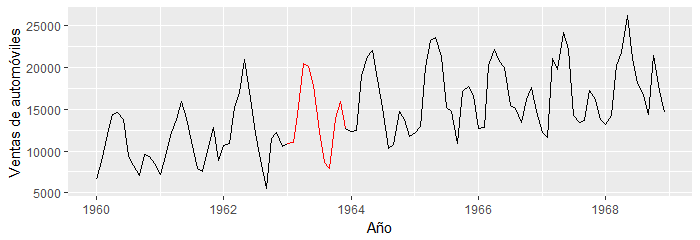
\includegraphics[scale = 0.7]{Images/Estructura/window.png}}
    \caption{Selección de las observaciones correspondientes a 1963 de la serie de ventas mensuales de automóviles en Quebec}
    \label{window}
\end{figure}

Es posible unir varias series temporales en un mismo objeto, para ello se suele recurrir al método $\verb!cbind()!$. La clase de este nuevo objeto pasa a ser $\verb!mts!$ que no es más que la clase $\verb!ts!$ extendida a series multivariantes.

Existen varios métodos más enfocados a realizar operaciones sencillas sobre series temporales que serán abordados en los apartados correspondientes a las librerías $\verb!zoo!$ y $\verb!xts!$ (aunque se aplican sobre objetos de clases distintas suelen presentar un comportamiento y una sintaxis similar).


\section{Zoo Package}
A diferencia de $\verb!stats!$, esta librería permite una estructuración de los datos más avanzada llegando incluso a poder almacenar series con intervalos de tiempo irregulares. La clase $\verb!zoo!$ combina el índice temporal y los datos en un mismo objeto facilitando así su tratamiento. La función encargada de estructurar los datos es $\verb!zoo()!$:
\begin{Verbatim}[fontsize=\footnotesize]
zoo(x = NULL, order.by = index(), frequency = NULL)
\end{Verbatim}

En este caso debemos introducir un vector con los valores de la variable ordenados cronológicamente y una frecuencia (igual que en $\verb!ts()!$) o un vector con las fechas ya generadas. Una función muy útil para generar una secuencia de fechas es $\verb!seq.Date()!$. Aunque en ocasiones es más sencillo generar la serie a partir de $\verb!ts()!$, suele ser necesario utilizar clases más extendidas como $\verb!zoo!$. El método $\verb!as.zoo()!$ se encarga de realizar la conversión entre estos objetos \cite{zoo}.

Es posible generar fechas mensuales y trimestrales a partir de las funciones $\verb!yearmon()!$ y $\verb!yearqtr()!$. El vector de fechas introducido como argumento a $\verb!zoo()!$ a través de $\verb!order.by!$ suele ser un objeto de clase $\verb!date!$, $\verb!yearmon!$ o $\verb!yearqtr!$ aunque existen otros más complejos capaces de almacenar el factor tiempo a través de minutos, horas, etc.

Es posible extraer el índice y las observaciones de nuestras variables a través de las funciones $\verb!index()!$ y $\verb!coredata()!$. Esto es muy útil para algunos métodos más restrictivos respecto a los argumentos que acepta. Una de las ventajas de esta clase de objetos es la posibilidad de seleccionar observaciones a través de la fecha. Si tenemos una serie mensual ($\verb!sales!$) comprendida entre los años 1960 y 1968 y queremos conocer los valores correspondientes al año 1963 basta con ejecutar la siguiente sentencia:
\begin{Verbatim}[fontsize=\footnotesize]
sales[seq.Date(from = as.Date("1963-01-01"), to = as.Date("1963-12-01"), by = "month")]
\end{Verbatim}

Para combinar varias series temporales en un mismo objeto basta con usar $\verb!merge.zoo()!$. En caso de que el intervalo temporal sea distinto este método completa los datos faltantes con $\verb!NAs!$, ofreciéndonos así como salida un objeto $\verb!zoo!$ totalmente operativo conformado por las series iniciales.

El tratamiento de los $\verb!NAs!$ suele ser un tema delicado en el que los investigadores no acaban de ponerse de acuerdo. Esta librería contiene varios métodos enfocados a esta problemática:
\begin{itemize*}
  \item[$\bullet$] \PVerb{na.aggregate()}: Permite remplazar los  $\verb!NAs!$ a través de datos basados en funciones como la media.
  \item[$\bullet$] \PVerb{na.approx()}: Sustituye los $\verb!NAs!$ a través de una interpolación lineal.
  \item[$\bullet$] \PVerb{na.spline()}: Recurre a la interpolación cúbica de splines para remplazar los $\verb!NAs!$.
  \item[$\bullet$] \PVerb{na.fill()}: Nos permite sustituir los $\verb!NAs!$ por los valores que queramos. Estos valores se introducen como vector a través del argumento $\verb!fill!$. También es posible la sustitución de los $\verb!NAs!$ a través de los valores adyacentes.
  \item[$\bullet$] \PVerb{na.locf()}:Sustituye los $\verb!NAs!$ por su valor más cercano en el tiempo. Es una implementación más directa del método anterior.
\end{itemize*}

Es posible retrasar la serie hacia delante o hacia atrás en el tiempo gracias al método $\verb!lag()!$:
\begin{Verbatim}[fontsize=\footnotesize]
lag(x, k = 1, na.pad = FALSE,...)
\end{Verbatim}

El objeto $\verb!zoo!$ se introduce al partir del argumento $\verb!x!$ y el rezago que deseamos aplicar a la serie a partir de $\verb!k!$. Es importante activar $\verb!na.pad!$ para no perder las fechas vinculadas al retardo $k$, ya que lógicamente con este retraso perderemos $k$ observaciones. Si $\verb!k!$ es positivo desplazamos la serie hacia delante y si es negativo hacia atrás.

Es posible utilizar $\verb!plot()!$ con objetos $\verb!zoo!$ para visualizar la evolución de la serie temporal. Al tratarse de la función $\verb!plot()!$ la sintaxis es similar a la que se suele usar normalmente para representar otros objetos más comunes en $\textsf{R}$. Esta librería contiene algunos métodos más completos para estos propósitos como puede ser $\verb!plot.zoo()!$ que facilita enormemente la representación de series temporales multivariantes.

Existen métodos que facilitan la lectura de datos. Lo más común es leer los datos desde un archivo $\verb!.csv!$ o $\verb!.txt!$ para almacenarlos en un $\verb!data.frame!$ y a partir de ahí realizar las transformaciones necesarias a fin de almacernarlos en un objeto $\verb!zoo!$. Los métodos $\verb!read.zoo()!$ y $\verb!read.csv.zoo()!$ nos ahorran este proceso y nos permiten pasar directamente de la lectura al objeto $\verb!zoo!$. En ocasiones es conveniente pasar a la función algún método a través del argumento $\verb!FUN!$ para tratar las fechas del archivo de origen .

En ocasiones nos puede interesar aplicar cierta función a nuestra serie de forma gradual, es decir, por grupos de observaciones. El método usado para este tipo de tareas es $\verb!rollapply()!$:
\begin{Verbatim}[fontsize=\footnotesize]
rollapply(data, width, FUN, align)
\end{Verbatim}

El argumento $\verb!data!$ recoge nuestro objeto $\verb!zoo!$ y $\verb!width!$ el número de observaciones sobre el que vamos a ir pasando la función recogida en $\verb!FUN!$. El argumento $\verb!align!$ nos permite decidir dónde queremos que empiece la ordenación cronológica del objeto $\verb!zoo!$ resultante. Por ejemplo, si tenemos:
\begin{Verbatim}[fontsize=\footnotesize]
rollapply(sales, 12, sum, align = "right")
\end{Verbatim}

Lo que realmente estamos haciendo es:
\begin{Verbatim}[fontsize=\footnotesize]
         sum(sales[1:12])
         sum(sales[2:13])
         sum(sales[3:14])
         ...
\end{Verbatim}

El resultado será un objeto $\verb!zoo!$ con una observación menos al final de la serie. El argumento $\verb!by!$ nos va a permitir aplicar la función elegida a cada intervalo de longitud $\verb!by!$ sin repetir observaciones.

Un método derivado de este último es $\verb!rollmean()!$. Gracias a él podemos suavizar nuestra serie a través de una media móvil de orden $k$. Para asegurarnos de que el cálculo se realiza únicamente con las observaciones pasadas debemos indicar que $\verb!align = "right"!$. Por ejemplo, para aplicar una media móvil de orden 12 que solo realice los cálculos con las observaciones de momentos ya transcurridos debemos escribir:
\begin{Verbatim}[fontsize=\footnotesize]
rollmean(x = sales, k = 12, align = "right")
\end{Verbatim}

Se puede apreciar fácilmente que es posible implementar $\verb!rollmean()!$ a través de $\verb!rollapply()!$. Para decidirnos por una u otra vamos a medir el tiempo de ejecución de cada una y para ello utilizaremos el método de la base de $\textsf{R}$ $\verb!system.time()!$. Este método toma como entrada una expresión a evaluar y nos devuelve tres valores:
\begin{itemize*}
  \item[$\bullet$] \textbf{User time}: Tiempo de ejecución llevado a cabo en la CPU.
  \item[$\bullet$] \textbf{System time}: Tiempo de ejecución llevado a cabo en el sistema operativo (lectura de datos, control de tiempos…)
  \item[$\bullet$] \textbf{Elapsed time}: Tiempo total transcurrido en la ejecución desde que se inició el proceso. Este tiempo es el que se utiliza para hacer el \textit{timing} del proceso.
\end{itemize*}

Para medir el tiempo de ejecución de cada método hemos generado una serie temporal con $10^5$ observaciones generadas a partir de una distribución normal con media 200 y desviación típica 20. A continuación se muestra el código empleado:
\begin{Verbatim}[fontsize=\footnotesize, numbers = left]
data <- zoo(rnorm(100000, 200, 20))
system.time(rollmean(x = data, k = 12, align = "right"))
system.time(rollapply(data = data, width = 12, FUN = mean, align = "right"))
\end{Verbatim}

El tiempo de ejecución en segundos llevado a cabo por $\verb!rollmean()!$ y $\verb!rollapply()!$ respectivamente es:
\begin{Verbatim}[fontsize=\footnotesize]
user  system elapsed
0.20    0.00    0.21

user  system elapsed
0.22    0.00    0.22
\end{Verbatim}

Como se puede apreciar estamos obteniendo tiempos similares. Para conseguir apreciar mejor la diferencia entre los métodos vamos a llevar a cabo una simulación. Ejecutaremos los dos métodos 100 veces para cantidades distintas de datos y después tomaremos la media de los tiempos para intentar eliminar el ruido inherente a la medición de los tiempos, los resultados se muestran en la Figura \ref{times_1}. Se puede ver como para números moderados de observaciones ambos se comportan parecido pero para números grandes $\verb!rollapply()!$ parece funcionar mejor que $\verb!rollmean()!$.

\begin{figure}
    \centering
    \centerline{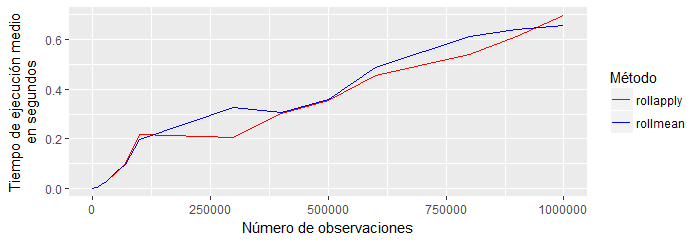
\includegraphics[scale = 0.7]{Images/Estructura/timing-roll.png}}
    \caption{Comparación de tiempos de ejecución para los métodos \PVerb{rollapply()} y \PVerb{rollmean()}}
    \label{times_1}
\end{figure}

\section{XTS Package}
Esta librería introduce una nueva clase de objetos conocida como $\verb!xts!$. Esta clase está basada en $\verb!zoo!$ pero tiene la gran peculiaridad de ser totalmente extensible a cualquier otra clase de datos temporales en $\textsf{R}$, es decir, da igual el formato en el que tengamos nuestros datos ya que siempre va a ser posible transformarlos a la clase $\verb!xts!$ \cite{xts}.

Al igual que con $\verb!zoo!$, para crear un objeto $\verb!xts!$ se debe usar el método $\verb!xts()!$ que se define de la siguiente manera:
\begin{Verbatim}[fontsize=\footnotesize]
xts(x = NULL, order.by = index(x), frequency = NULL, unique = TRUE,…)
\end{Verbatim}

Lo realmente interesante de este paquete es su capacidad de aunar cualquier estructura temporal. Existen muchos objetos capaces de almacenar nuestros datos ($\verb!ts!$, $\verb!zoo!$, $\verb!timeSeries!$, $\verb!matrix!$, $\verb!data.frame!$…) y todos ellos pueden ser convertidos a $\verb!xts!$ a través del método $\verb!as.xts()!$:
\begin{Verbatim}[fontsize=\footnotesize]
as.xts(x,...)
\end{Verbatim}

En un principio puede parecer inútil almacenar una serie temporal en un objeto $\verb!matrix!$ o $\verb!data.frame!$ pero es muy útil si se quiere trabajar con series temporales multivariantes.

Esta clase de objeto está equipada con un sistema de selección de observaciones realmente intuitivo y útil. A continuación mostraremos un ejemplo de esta característica aplicada a una nuestra serie mensual $\verb!xts.sales!$:
\begin{Verbatim}[fontsize=\footnotesize, numbers = left]
# diciembre de 1963
xts.sales["1963-12"]
# el año completo de 1963
xts.sales["1963"]
# todas las observaciones hasta julio de 1963
xts.sales["/1963-7"]
# todas las observaciones a partir de julio de 1963
xts.sales["1963-7/"]
# observaciones comprendidas entre julio de 1962 y de 1963
xts.sales["1962-7/1963-7"]
\end{Verbatim}

Al ser $\verb!xts!$ una extensión de $\verb!zoo!$ todos los métodos de este último se pueden aplicar al primero sin necesidad de modificar las entradas de los argumentos. Algunos de estos métodos como $\verb!index()!$ o $\verb!merge()!$ detectan la clase del objeto y se adaptan a él ejecutándose automáticamente como $\verb!index.xts()!$ y $\verb!merge.xts()!$.

Esta librería incluye también métodos bastante más avanzados para el tratamiento de formatos y estructuras, razón por la cual los analistas más expertos se suelen decantar por ella.

Existen también un conjunto de métodos para objetos $\verb!xts!$ encargados de iterar a través de series y aplicar funciones a conjuntos de observaciones determinadas. Todos ellos se sustentan en $\verb!period.apply()!$:
\begin{Verbatim}[fontsize=\footnotesize]
period.apply(x, INDEX, FUN, …)
\end{Verbatim}

El objeto $\verb!xts!$ se pasa a través de $\verb!x!$, la función a aplicar a través de $\verb!FUN!$ y el índice de las observaciones a través de $\verb!INDEX!$. A diferencia de $\verb!rollapply()!$ en este caso no pasamos el número de observaciones sino el índice de estas. Un método muy útil para seleccionar los índices deseados es $\verb!endpoints()!$, este método extrae los índices correspondientes a las últimas observaciones de un periodo dado. Por ejemplo, si queremos obtener una subserie ($\verb!subserie.1!$) formada por las medias anuales de la serie $\verb!xts.sales!$ basta con escribir:
\begin{Verbatim}[fontsize=\footnotesize, numbers = left]
subserie.1 <- period.apply(x = xts.sales,
                           INDEX = endpoints(xts.sales, on = "years"), FUN = mean)
\end{Verbatim}

Y con lo dicho anteriormente tenemos que:
\begin{Verbatim}[fontsize=\footnotesize]
subserie.1[1] == mean(xts.sales["1960"]) # TRUE
\end{Verbatim}

Existen también variaciones de $\verb!period.apply()!$ orientadas a la optimización de funciones usualmente aplicadas a series temporales como son $\verb!period.max!$, $\verb!period.min!$, $\verb!period.prod!$ y $\verb!period.sum!$.

Normalmente se suele trabajar con series diarias, mensuales, cuatrimestrales o anuales así que con el formato $\verb!ts!$ bastaría. Sin embargo hay ocasiones en las que el tiempo se estrucutra de forma más complicada, en esos casos conviene utilizar $\verb!zoo!$ o $\verb!xts!$. Esta última suele estar recomendada para profesionales que trabajan con series estructuradas bajo intervalos temporales con formatos irregulares.




